\section{Vanishing line}

The objective of this task is to determine the vanishing line, denoted as $\mathbf{l}^\prime_{\infty}$ of the horizontal plane. 
The horizontal plane is formed with the width and depth of the object.
\begin{figure}[H]
    \centering
    
\includegraphics[width=0.75\linewidth]{images/cropped.jpg}
    \caption{Original image}
\end{figure}
The lines on the width and the depth of the object from now on will be called $\mathbf{l}_i$ and $\mathbf{m}_j$, respectively.

\subsection{Vanishing points}
To determine the vanishing points, we need to identify the intersection of two lines that are parallel in the real world but appear to converge in the image.
This can be done thanks to the following theorem:
\begin{theorem}
    The image of a set of parallel lines $\mathbf{n}_i$ is a set of concurrent lines $\mathbf{nl}^\prime_i$ that intersect at a common point $\mathbf{p}^\prime$, referred to as the vanishing point of the direction of lines $\mathbf{n}_i$. 
\end{theorem}

For both the width and depth, we select two pairs of points that lie along the same line. 
To derive the equation of the line passing through two points, we compute the cross product in the 2D plane.
In general, given two points $\mathbf{x}_1$ and $\mathbf{x}_2$, the line can be expressed as:
\[\mathbf{l}=\mathbf{x}_1 \times \mathbf{x}_2\]
By performing this operation for four pairs of points, we obtain two lines for each dimension:
\[\mathbf{lh}_1 \qquad \mathbf{lh}_2 \qquad \mathbf{lm}_1 \qquad \mathbf{lm}_2\]

The vanishing point for each dimension is found by intersecting the respective lines. 
This can be done by taking the cross product of the two lines:
\[\mathbf{p}_l=\mathbf{lh}_1 \times \mathbf{lh}_2\]
\[\mathbf{p}_m=\mathbf{lm}_1 \times \mathbf{lm}_2\]
\noindent In the given image, we ha found the following vanishing points:
\begin{figure}[H]
    \centering
    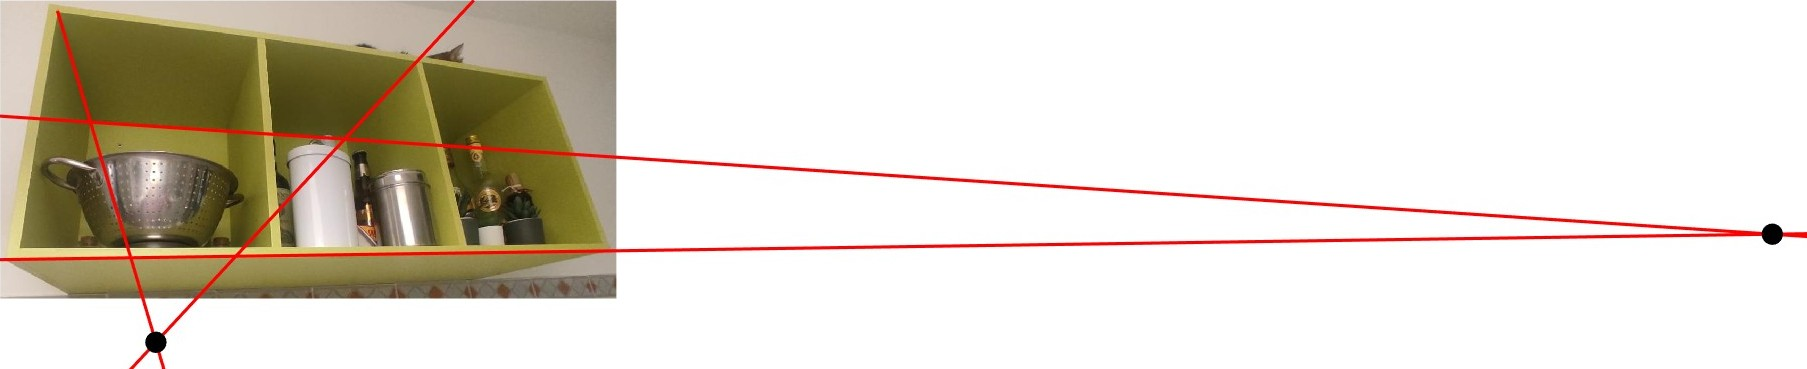
\includegraphics[width=1\linewidth]{images/vanishing_points.jpg}
    \caption{Vanishing points for depth and width}
\end{figure}
The coordinates of the vanishing points are given by:
\[\mathbf{p}_l=\begin{bmatrix} x_l \\ y_l \\ w \end{bmatrix} \qquad \mathbf{p}_m=\begin{bmatrix} x_m \\ y_m \\ w \end{bmatrix}\]

\subsection{Vanishing line}
The vanishing line $\mathbf{l}^\prime_{\infty}$ is defined by the connection between the two vanishing points, $\mathbf{p}_l$ and $\mathbf{p}_m$. 
This is achieved by computing the cross product of the two points:
\[\mathbf{l}^\prime_{\infty}= \mathbf{p}_m^T \times \mathbf{p}_l^T=\begin{bmatrix} a \\ b \\ c \end{bmatrix}\]
\noindent In the given image, we ha found the following vanishing line:
\begin{figure}[H]
    \centering
    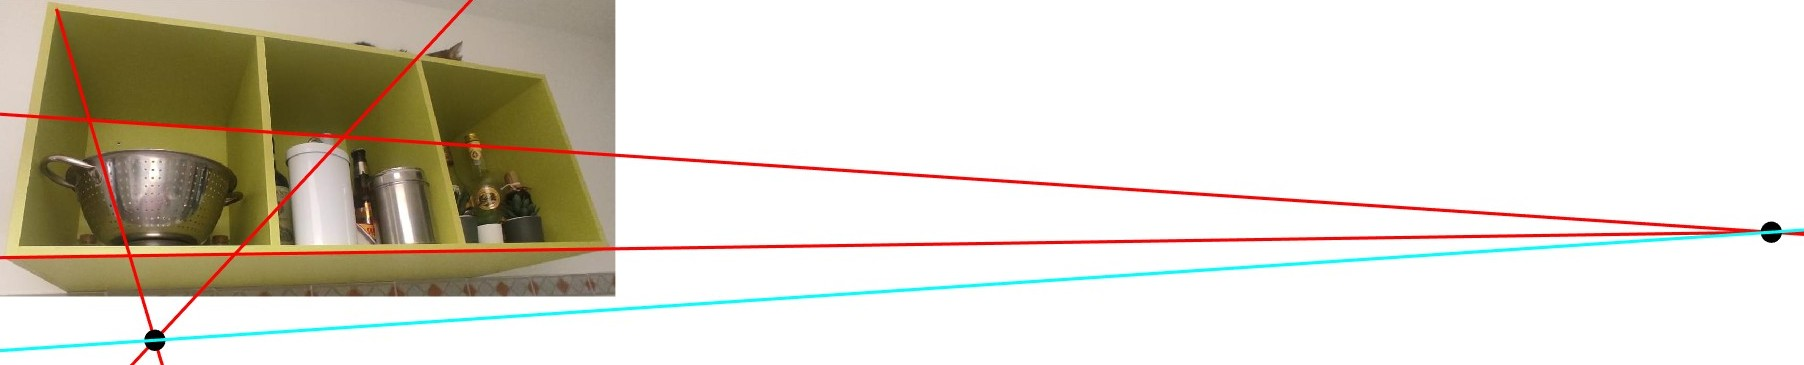
\includegraphics[width=1\linewidth]{images/vanishing_line.jpg}
    \caption{Vanishing line for depth and the width dimension}
\end{figure}